\documentclass[ProjectRequirements.tex]{subfiles}
\begin{document}

\bigskip

\section{\textsc{\Large Overall Description}}
	\subsection{Product Perspective}
	\begin{figure}[H]
		\centering
		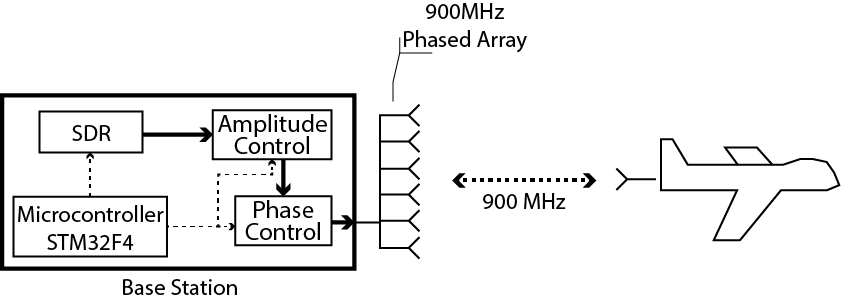
\includegraphics[]{HardwareBlockDiagram.png}
		\caption{Hardware Block Diagram \label{fig:HardwareBlockDiagram}}
	\end{figure}
	\begin{figure}[H]
		\centering
		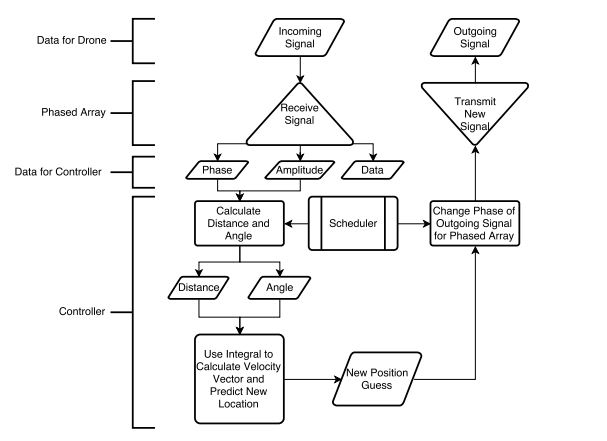
\includegraphics[]{SoftwareBlockDiagram.png}
		\caption{Tracking Block Diagram \label{fig:SoftwareBlockDiagram}}
	\end{figure}
			
		\subsubsection{User Interfaces}
			The system must have an Ethernet port through which the user can establish a connection. The user should be able to modify various settings and send the commands of interest through this port. This port must conform to the following requirements:
			\begin{enumerate}
				\item When a connection is established, the interface must send a list of instructions and changeable parameters over Ethernet.
				\item The interface must be straightforward enough that a technical user can use the instructions to configure the settings within 20 minutes.
				\item There must be clear documentation about each setting describing (1) what it does, (2) why it's valuable, and (3) how to use it.
			\end{enumerate}	
			
		\subsubsection{Hardware Interfaces}
			\begin{enumerate}\itemsep1pt
				\item \textbf{STM32F4} -- 
				\item \textbf{Xeta SDR} -- 
				\item \textbf{Phased Array} -- 
			\end{enumerate}
			
		\subsubsection{Software Interfaces}
			\begin{enumerate}\itemsep1pt
				\item Tracking interface
				\item 
			\end{enumerate}
			
		\subsubsection{Communications Interfaces}
			\begin{itemize}\itemsep1pt
				\item 
			\end{itemize}
			
		\subsubsection{Memory}
			\begin{itemize}\itemsep1pt
				\item 
			\end{itemize}
		
		\subsubsection{Operations}
			\begin{itemize}\itemsep1pt
				\item 
			\end{itemize}
		
	\subsection{Product Functions}
	
		\subsubsection{High Priorities}
			\begin{enumerate}
				\item \textbf{Distance} -- The 900MHz phased array must be able to establish a connection with a drone in motion up to 20 miles away. A connection will be considered valid if we are receiving packets with our header on them every second.
				\item \textbf{Power} -- The 900MHz phased array must never exceed the FCC maximum power specifications, which is 4 watts.
				\item \textbf{Command Transmission Rate} -- The 900MHz phased array must be able to transmit telemetry at 10Hz.
				\item \textbf{Cost} -- The project should cost no more than \$10,000 to produce the prototype
							
			\end{enumerate}
		
		\subsubsection{Medium Priorities}
			\begin{enumerate}
				\item \textbf{Communications} -- The communications should be radio agnostic.
				\item \textbf{Stacked Antennas} -- The 2.4GHz phased array must be able to establish a connection with a drone in motion up to 5 miles away.
			\end{enumerate}
		
		\subsubsection{Low Priorities}
			\begin{enumerate}
				\item \textbf{Multiplexing} -- The phased arrays should be able to simultaneously communicate with up to 4 drones at once while maintaining a lock.
				\item \textbf{Video} -- The 
			\end{enumerate}
		
	\subsection{User Characteristics}
		We intend to market this product to people who are interested in managing multiple drones at once with lower power at longer distances. Because this is a backend product, the user will be expected to be somewhat familiar with embedded systems. The user should have prior knowledge of SDR and drones. Because the system is radio agnostic, the user will need to supply his own SDR. The user will need to supply data that is compatible with his SDR to our program.\\
		
		The user will not be expected to have familiarity with RF Design, tracking, locking, or our internal headers.
		
	\subsection{Design Constraints}
	
	\subsection{Assumptions and Dependencies}
	
\end{document}
